\newpage
\subsection{ALS Chain}
\textit{ALS Chains} sind die Verallgemeinerung von \textit{ALS XZ} und \textit{ALS XY Wing}. Ein \textit{ALS XZ} ist eine \textit{ALS Chain} der Länge 2 und ein \textit{ALS XY Wing} ist eine \textit{ALS Chain} der Länge 3. Eine \textit{ALS Chain} ist eine Kette von {ALS} verbunden durch \textit{RCCs}, für die gilt, dass keine zwei aufeinanderfolgenden \textit{RCCs} gleich sein dürfen. Die \textit{ALS} am Anfang und Ende der Kette enthalten eine gemeinsame Ziffer Z. Diese Ziffer wird wie gewohnt dann aus allen Kandidatenlisten gelöscht, die von allen Instanzen der Ziffer Z im \textit{ALS} am Anfang und am Ende der Kette gesehen werden.\\
Das geht, da durch die Verknüpfung durch \textit{RCCs} die Ziffer Z entweder im \textit{ALS} am Anfang der Kette stehen muss oder in dem am Ende.

\begin{figure}[h]
\begin{center}
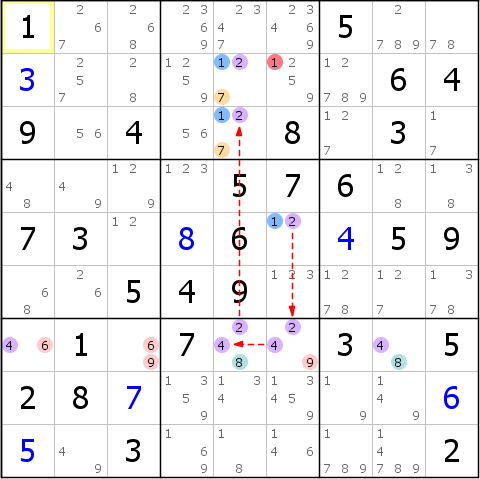
\includegraphics{./img/ALS_Chain.png}
\caption{ALS Chain}
\end{center}
\end{figure}

In \textbf{Abbildung 4.20} sieht man eine \textit{ALS Chain} der Länge 4. Das erste \textit{ALS} ist in Zeile 2 Spalten 1, 2, 4 und 9, es enthält die Kandidaten 2, 3, 5, 6 und 7. Durch den \textit{RCC} 7 ist es verbunden mit dem einzelligen \textit{ALS} in z2s7, das die Kandidaten 3 und 7 enthält. Dieses \textit{ALS} ist durch den \textit{RCC} 3 verbunden mit dem \textit{ALS} in z7s7, wiederum mit den Kandidaten 3 und 7. Die letzte Verbindung besteht dann durch den \textit{RCC} 7 zum \textit{ALS} in Block 8 mit z7s4 und z8s5, das die Kandidaten 2, 3 und 7 enthält. Das erste und das letzte \textit{ALS} enthalten den gemeinsamen Kandidaten 3. Dieser kann nun als Kandidat aus allen Zellen gelöscht werden, die alle Instanzen der Ziffer 3 in beiden \textit{ALS} sehen. Das ist der Fall in z8s4 und z9s4.